\documentclass[11pt,a4paper,oneside]{article}
\renewcommand{\baselinestretch}{1.2}
\usepackage{sectsty,setspace,natbib,wasysym} 
\usepackage[top=1.00in, bottom=1.0in, left=1in, right=1.25in]{geometry} 
\usepackage{graphicx}
\usepackage{latexsym,amssymb,epsf} 
\usepackage{epstopdf}
\usepackage{amsmath}
\usepackage{natbib}

\newenvironment{smitemize}{
\begin{itemize}
  \setlength{\itemsep}{1pt}
  \setlength{\parskip}{0pt}
  \setlength{\parsep}{0pt}}
{\end{itemize}
}

\usepackage{fancyhdr}
\pagestyle{fancy}
\fancyhead[LO]{December 2013}
\fancyhead[RO]{Variable environments \& climate change}

\begin{document}
\renewcommand{\labelitemi}{$-$}
\title{Coexistence and climate change: \\The role of
    temporal-variability in structuring future communities}
    \author{Wolkovich \& Donahue}
\date{Last updated: 11 December 2013}
\maketitle

\begin{abstract} Predicting community shifts
with climate change requires fundamental appreciation of the
mechanisms that govern how communities assemble. Most work to date has
focused on how warmer mean temperatures may affect individual species
via physiology, generally producing range shifts towards the poles and
uphill, which fails to predict the wide diversity of observed shifts.
Climate change has and is expected to affect far more than mean
temperatures, including widespread affects on growing season
length, variability and shifts in extreme events. Additionally,
cascading effects on species and communities are qualitatively
predicted but there have been no efforts, to our knowledge, to predict
shifts based on coexistence theory. Here we extend the two possible
mechanisms for species coexistence based on variable environments---
relative nonlinearity and the storage effect---to predict how
communities will respond to climate change. We focus on both (1) shifts in
climate variability and extreme events that link to
stabilizing coexistence mechanisms and (2) traits that may
make species the most vulnerable to climate change. We examine how
coexistence via the storage effect shifts under non-stationary climate regimes, and how outcomes vary with the
ability of species to phenologically track the timing of major climate events. \emph{Findings go here. Such as: Species that can track variability are least vulnerable to climate change (perhaps).  Also, we add an emphasis on integrating intra and inter-annual scales here, if we manage to make that happen well.}
\end{abstract}

\newpage




\section{Next steps, goals!}
\noindent World of possibilities goes here soon.

\section{Introduction}
\noindent \emph{Need to write more someday} \\
\noindent Understanding how plant communities will respond to climate change
requires synthesizing information on both direct effects of climate on species
and indirect effects driven by responses to other species'
shifts. (Coexistence models based on variable environments allow us to
do this, as species respond to shifting resources, which are
influenced both by abiotic stressors and the use of the resource by
other species.)

\section{Overview of project and directions}
\noindent 
\begin{enumerate}
\item We consider the effects of climate variation at both the
intra-annual and inter-annual scale and scale up responses to
short-term (1-10 yr?) and long-term (\(>\)100 yr) dynamics. 
\item We focus (for now) only on the storage effect. We leave out relative non-linearity.
\item We also look at how species traits related to their responses to
  climate variability effect coexistence and long-term diversity
  maintenance. (This is the tracking part of the project.) 
\end{enumerate}

\noindent We also note that one possible way to make this project more
interesting, useful and forward-thinking than others is to make
scenarios most realistic---link to real climate scenarios or use
existing data to rule out and in shifts in abiotic variables (and
possibly species traits---we should have the data to estimate the
percentage of species that track, maximum tracking and if only
early-season species track, we could add that in, and of course we
have a lot of climate data on hand). The new \emph{Physical Sciences Basis} of the IPCC came out in September 2013 so we have good recent estimates of how climate has and will shift (and Lizzie can slog through this).

\section{Current outline}
\begin{enumerate}
\item Introduction
\begin{enumerate}
\item Direct and indirect effects of climate change
\item Links to ecological coexistence theory
\item Abiotic shifts expected with climate change: single versus
  synergistic climate shifts
\item Things that will shift with climate change, related to
  coexistence models
\begin{enumerate}
\item Magnitude of and interannual variance in resource pulse (\(R_{\theta}\))
\item Timing of resource pulse (\(\tau_{p}\))
\item Abiotic loss rate of resource (\(\epsilon\))
\end{enumerate}
\item Species traits and climate change: phenological tracking
\item Goals of paper
\end{enumerate}
\item Model description (a whole section on this below)
\begin{enumerate}
\item Basic storage effect model
\item Our version of the storage effect model
\item Systems for which model is applicable: This is effectively a system with a single large pulse of
resource, that, in a plant-free scenario is lost exponentially each
year. 
\begin{enumerate}
\item Alpine systems (resource is water): initial large pulse of precipitation from
  snowpack that gradually is used up  throughout season
\item Arid systems? (resource is water): Major pulse of rains (okay, spread out some,
  but really they often concentrate for a couple months and then
  season continues for 3-4 more months)
\item Temperate systems (resource is nutrients): Work with me here, I
  think this is cool. Early in the season turnover of microbes leads
  to a huge flush of nutrients \citep{Zak:1990ar} that microbes (and plants) draw down
  all season. There's no other pulse really---am I crazy here or
  doesn't this work well? (And so microbes draw it down in the
  plant-free case which could easily be affected by climate change,
  e.g., increased temperatures lead to increased microbial activity
  and more rapid draw-down.)
\end{enumerate}
\item Systems it probably doesn't work for: Light-limited systems
  (there is not a single, plant-free decreasing pulse of resource),
  Great Plains or others with multiple pulses.
\item Phenological tracking and the storage effect
\item Our implementation of tracking
\item Derivation of aspects of the storage effect and relative
  non-linearity in our model (this is a big \emph{to do}).
\end{enumerate}
\item Results: Response variables are (1) probability of extinction,
  (2) relative
  densities in 2 spp models, and as of 2012-2013, what are the traits of species that persist? How much of a trade-off is needed to offset shifts in coexistence favouring early or tracking species with non-stationary climate change?\\
\begin{enumerate}
\item Section 1: Shifting abiotic variables
\item Section 2: Species traits: Phenological tracking and shifting
  abiotic variables
\end{enumerate}
\item Discussion
\end{enumerate}

\section{Variables of interest}
We consider 3 primary traits of the environment (\(\epsilon, R, \tau_{p}\), which
code to evaporative stress, inter-annual variability, and start of season pulse for our approach basically) and 1
species response trait (phenology, specifically flexibility in
phenology as modeled by a species' ability to shift \(\tau_{i}\)) to model
the dominant expectations of current and future climate change:
\begin{enumerate}
\item \emph{Changes to R:} Shifts in climate means and variability (greater var \(\approx\)
  extreme events) as modeled by changes to \(\mu\) and \(var\) of
    R,
  which can lead to:
\begin{enumerate}
\item Changes in inter-annual covar(E, C)
\item We ignore, for now, possible changes related to this in relative non-linearity
\item For variability: changes related to buffered population growth:
  for example, when the periodicity of certain extreme events declines
  such that species with certain buffering times no longer get their
  `good' years enough (e.g., periodicity of rainy years every 5 years,
  switches to 10 and the species seedbank is 7 years). This means for
  simulations changing \(var(R)\) must be consider in concert with the
  scale of \(s_{i\cdots n}\).
\end{enumerate}
\item \emph{Changes to \(\epsilon\):} Shifts in climate means that lead to greater abiotic stress on
  environments, as modeled by changes to  \(\epsilon\). For example,
  warmer growing seasons may produce greater evapotranspiration,
  shifting competition for the remaining resource. (By the way, we
  have notes about treating \(\epsilon\) as a function itself.) This should
  affect:
\begin{enumerate}
\item Changes in inter-annual covar(E, C)
\item We ignore, for now, possible changes related to this in relative non-linearity
\end{enumerate}
\item \emph{Changes to \(\tau\):} Longer growing seasons, with several scenarios:
\begin{enumerate}
\item Season is longer (earlier \(\tau_{p}\) but community of species
  do not shift their timing (e.g., no change to  \(\tau_{i \cdots
    n}\)) 
\item Season is longer (earlier \(\tau_{p}\) and some species (`climate-trackers') change
  their timing (community shift in temporal (phenological) synchrony),
  that is (e.g., certain species change to  \(\tau_{i \cdots
    n}\)) such that the distance \(\tau_{p}-\tau_{i}\) is constant
  across years.
\item Could also look at complementarity (histogram of variation in \(\tau_{i \cdots
    n}\); could pull \(\tau_{i \cdots
    n}\) from a beta distribution. (Note: I also wonder if we
  shouldn't just use variation due to above to look at this, versus a
  whole new approach.)
\end{enumerate}
\item How do these variables shift with climate change and co-vary?
\begin{enumerate} 
\item \(R_{\theta}\) increasing inter-annual variance with some giant
  years (extreme events), for snowpack systems it's decreasing
  generally
\item \(\tau_{p}\) getting earlier, also for snowpack systems earlier
  years probably also have higher evaporative stress (\(\epsilon\),
  due to warmer year)
\end{enumerate}
\end{enumerate}

\noindent We assume that:
\begin{enumerate}
\item All species `go' each year, at least a little; that is, we're
  not looking at a communities where some species have true
  supra-annual strategies.
\item There is one dominant pulse of the limiting resource (e.g.,
  light or water) at the
  start of each growing season; thus we model a  single pulse per
  season.
\item While interactions between the above-considered `traits' may be
  important, first understanding how each of these forces act alone is
  critical enough to let alone interactions for this manuscript.
\end{enumerate}

\subsection{Tracking thoughts \& fun}
In August 2012 Megan came up with a new way to model phenological tracking, it's linear and better than the one presented here. We also discussed three key ways to think of tracking:
\begin{enumerate}
\item Species can have fixed flowering/leafing (not track).
\item Species can phenologically track pulse.
\item Species can phenologically track something at least at one time in history correlated with the pulse.
\end{enumerate}
We agreed that while (3) is interesting---would allow you to look at mismatch ideas etc.---(1) and (2) have more biological support for plants and are interesting enough in and of themselves, so we will focus on and mode (1) and (2) and not (3).\\

\noindent In August 2013 an issue we worried about: Will tracker always win? Answers: No, not if it's a poor competitor, that is, if it responds quickly to resource pulse but then does poorly at low resource levels. I also think it's important to remember that not all tracking species will track perfectly so some species should grow before trackers some years, when their fixed \(\tau_{i}\) corresponds well to \(\tau_{p}\). Also, we have a note high intraspecific competition could dampen trackers, especially when greater than interspecific competition.\\

\noindent New things we came up with that we want to look at in regards to {\bf phenological tracking}:
\begin{itemize}
\item How big do trade-offs have to be for tracking to be non-advantageous (to allow coexistence with other species)?
\item Has climate change made tracking more advantageous? That is, is tracking the dominant strategy with a shifting environment (distribution) vs. stationary environment distribution?
\item Follow up from October: How much does climate have to shift (non-stationarity in system) given some level of fitness differences trading off with tracking for tracking to become the optimal strategy \emph{or, given that we know something about climate projections} how big do the trade-offs have to be with climate change to make non-tracking a feasible strategy strategy (that is, to make tracking not the optimal strategy with climate change)?
\end{itemize}

\noindent New notes as of October 2013:\\
\emph{How will we adjust the equations for simulations about shifts in the environment?\footnote{Not phenological tracking, which are other simulations.}'}
\begin{itemize}
\item We do {\bf not} have relative nonlinearity: So we set all species \(f(R)\) the same. 
\item We have to create some species differences for the storage effect to `ameliorate' (EMW phrasing here, probably not ideal), so how do we want to do that?
\begin{itemize}
\item mean species differences in \(c_{i}\) and storage effect through \(g_{i}\) 
\item mean species differences in \(g_{max,i}\) and make them totally equivalent within season and temporal storage effect through \(\tau_{p}-\tau_{i}\) 
\end{itemize}
\item Note: \(h\) yields different bet hedging strategies (you could think of it as `germination plasticity')
\item Question: do we need to make sure that for all \(i\), \(\int g_{i}\) are equal, or is it that \(\int g_{i}(t)\tau_{p}(t)\mathrm{d}t\) should be constant (the latter being the average of \(g_{i}\) weighted by the distribution of \(\tau_{p}\) through time).
\end{itemize}

\noindent \emph{New notes on trade-offs from 12 November 2013:}\\
In nature early species have quicker-return-investments on growth and early is often high tracking, so it's hard to tell whether early \emph{or} high-tracking trades off with this quicker-return angle. So what we plan on doing:\\

\noindent For now, for coexistence: we'll trade off \(c_{i}\) and \(\tau_{i}\), when we add in alpha we'll leave this above trade-off and maybe:
\begin{itemize}
\item get some coexisting species and add high tracking randomly to all and see what happens
\item get some coexisting species and add high tracking to the early ones and see what happens
\end{itemize}

\noindent \emph{Megan's thoughts from the plane home:} Can think of trade-off as competition-colonization one: rapid response to resource availability (colonization) versus special case of competition.\\
{\bf Megan! We would all benefit if you fix my hack of the following:} Without tracking we may predict benefits to early-colonizers decline with earlier seasons. As start-date moves earlier, early folks lose benefit and you get more late folks. Late species may be less different than one another---and less responsive to environment. Early folks, effectively, become more similar to environment. 

\subsection{How the world changes with climate change}

\noindent In July 2011, I looked at whether the start of spring
has gotten more variable (using some key datasets from NECTAR) and it
hasn't, at all. No change.\\

\noindent Old list of tasks on this I should make sure are thought through:
\begin{itemize}
\item Get on top of climate change lit: which variables will shift?
  Which ones are coupled and how will their coupling shift with
  climate change (go from uncoupled to coupled, or vice-versa, or just
  the coupling itself changes)?
\item Does evaporative stress increase with climate change (absolute,
  versus relative, oceans burn off while temperatures increase etc.)?
\item When seasons start earlier does evaporative stress increase (I
  suspect so, but need to pull together refs)?
\item Does lower snowpack mean earlier seasons?
\end{itemize}

\noindent \emph{Environmental shifts with climate change, from October 2013 meeting:}\\
Systems we're thinking about (see above) but, effectively, alpine where snowpack meltout is start of season (SOS), nutrient turnover SOS and some precip controlled systems with just one pulse. 
\begin{enumerate}
\item \(\tau_{p}\) will get earlier in many systems (alpine and nutrient), not sure on precip---there it might just get more variable
\item \(\epsilon\) increase in mean and increase in extreme events (this seems pretty possible across a lot of systems---good one)
\item \(R_{0}\) increase or decrease in mean maybe (who knows what happens in precip system), increase in variance (for precip systems), increase in extreme events 
\item Correlations in \(\tau_{p}\) and \(\epsilon\) - this basically says `does the first day of the growing seeason correlate with the average temperature of the growing season?' which, yeah, is weird. Lizzie thinks there's probably a weak positive covariance here (just because there's a lot of noise in annual weather but wet soils hold cold, and dry soils hold heat so \emph{all other things being equal} you could see this correlation. From an email from Ben Cook from 30 May 2013:
\begin{quote}
So, both Europe and the Northeast US have had super crappy springs in March and April (so annoying!). Mostly it was due to an almost unprecedented negative swing of the NAO, which just funneled lots of cold arctic air in the region. As for the summer? Harder to tell. If an area gets lots of rain in the spring, it can mean really wet soil which can keep things cooler in the summer. But other than that, we don't really have much skill in predicting summer time climate. 
\end{quote}
Otherwise, not sure anyone has looked at this at all in precip systems and for snowpack there may be something here since Pederson et al. 2011 says that snowpack control has basically shifted from precipitation control to temperature control so with climate change you could start seeing a correlation in alpine systems between \(\tau_{p}\) and \(\epsilon\) (which is kind of cool, but sort of something that is not low-hanging, obvious fruit -- or maybe it's low hanging fruit and only obvious to us).
\item Correlations in \(\epsilon\) and \(R_{0}\) maybe for alpine you could see, with climate change, increases in \(R_{0}\)  and decreases in \(\epsilon\), but we're still bickering on this and what \(\epsilon\) really is (incident irradiance vs. relative humidity?)
\item Correlations in \(R_{0}\) and \(\tau\) nothing to date or in future? Maybe in alpine systems?
\end{enumerate}

So, where did we arrive at after all this? Even though we used to be interested in correlated shifts in these we're not so much anymore. Instead the \emph{best place to start} seems to be: earlier \(\tau_{p}\) and increases in \(\epsilon\) and \(\epsilon\) extreme events. Then maybe move on to \(R_{0}\) (mean and extreme events). And again, just skip correlations.\\

Note that increased extreme events for \(\epsilon\)  will effectively reduce biomass (you could also consider modeling this so it ties to \(m_{i}\) or modify \(g_{i}\) to lead to total loss, perhaps).\\

While here, though, I will mention that we discussed \emph{which} correlations will shift with climate change and the big one seems to be the North American alpine story: where the relationship between how \(\tau_{p}\) affects mortality has shifted with species' \(\tau_{i}\) such that there is now higher mortality imposed on species with earlier \(\tau_{i}\). We did briefly discuss how to model this and think maybe the best way is to add in, external to the within-year integral, a fraction that germinated and died as a f(x) of \(\tau_{i}\)  and frost event time.\\

\section{Random things to remember, worry over, generally absorb}

\noindent {\bf Key question:} Should we add asymmetry in \(g_{i}\) such that \(\tau_{i}\) earlier than \(\tau_{p}\) is worse than \(\tau_{i}\) later than \(\tau_{p}\)?\\

\noindent {\bf Key stuff:} We will build in trade-offs (versus running a bunch of random parameter space models where---in order to get stability---we end up with related trade-offs) such that we're effectively saying `the world works this way now, we add climate change and see what happens. . . .' We think these trade-offs should be:
\begin{itemize}
\item decrease \(\phi_{i}\) correlated with  \(\tau_{i}\) close to  \(\tau_{p}\)
\item (for phenological tracking questions) decrease \(\phi_{i}\) correlated with higher tracking\footnote{though we could also alter \(c_{i}\) or \(u_{i}\), or might work better to adjust \(a_{i}\) so you can make earlier faster growers (or adjust \(a_{i}/u_{i}\) so when you're faster you're a higher R*), but we need to check through all this thinking more.}
\end{itemize}

\noindent Remember to worry a little about how biomass is converted to seed: It happens for all species at $\delta$---so, early species may have peaked and have lower-than-their-peak biomass at $\delta$ while later season species may be at peak. Ways around this?\\

\noindent Use peak biomass instead of biomass at $\delta$ (when the growth rate goes below 0). \\

\noindent Set different $\delta$ for each species ($\delta_{i}$)\\

\noindent \emph{The way the growing season ends in the equations is
interesting.} First, as brilliantly stated: the growing seasons ends
[in these equations] when plants stop growing. And related, the
equations do not deal with setting the end of the growing season. In
my head (Lizzie), abiotic forces can stop a growing season, but in
reality with plant phenology data, the start and end of the growing
season are fundamentally different: at the start species are most
sensitive to abiotic cues and climate change effects are large and
often consistent. For the end of the season effects have been more
muted and variable---suggesting plants in someway do seem to set the
end of the growing season more than abiotic cues do, at least when
compared to the start of season. (And the model follows this.)\\

Worries over growing season continue (from August 2012 notes)! Worries over very short growing seasons (agree to stay with what we have for now, but keep in mind this possible issue and idea of continuous $R$ dripping in (or cyclically) for `growing season').\\

\noindent The intra-annual model does not have a useful closed solution (I
  have some Maxima code that shows only the trivial solution gives an
  equilibrium). This actually makes sense since the model is not a
  chemostat (a la Tilman \(R^{*}\)), we have a pulse that drains out
  and is not balanced by inputs.\\

\noindent {\bf Key question:} Can we simplify within-year dynamics to focus on a better model for timing (see photo of October 2013 whiteboard that Megan has)? To rephrase this: Our internal equation is basically R* rankings could we create a `deterministic look up table' for the within-year dynamic so we can make think more carefully about the timing part of this.  (Related note from 2012 meeting: Decide if we need to ODE solve the intra-annual
  dynamics, then use the discretized version only inter-annually. Note from Lizzie: best ODE solver is now in package `desolve.')\\

\noindent The 3 ingredients of the storage effect are:
\begin{enumerate}
\item differential response to the environment (subadditivity)
\item covar(E, C)
\item buffered population growth
\end{enumerate}

\noindent Ingredients for the storage effect \emph{in our model:}
\begin{itemize}
\item buffered population growth: \(s_{i}\)
\item variable response to the environment: \(\tau_{i}\), which generates:
\item \(covar(E,C)\)
\end{itemize}

\(\tau_{p}\) is conceptualized as a photoperiod cue, it's a species going on the same day every year---for our phenological tracking we adjust it so it can vary year-to-year for some species.\\


\noindent We keep an eye on who has cited Chesson et al. 2004
and for actual modeling work it's just Chesson, and for that it's all
his seed predation work.\\

\noindent More random notes: \citet{Chesson:2000vd} (pg. 354) \(r\) holds temporal variation in \(\delta I\) and \(\delta N\) so effectively:\\
- species can coexist via intra-annual temporal mechanisms (for example, maybe this is what most mid-season species in the mesic temperate zone do), and/or\\
- species can coexist via inter-annual temporal mechanisms (maybe early-season species in most mesic temperate environments)\\


\noindent {\bf Some notes for writing}
\begin{enumerate}
\item Understanding the variable responses of communities and species
  due to climate shifts is a major aim of current
ecology.
\begin{enumerate}
\item Varied responses
\begin{enumerate}
\item reversed phenology \citep{yu2010} 
\item downhill shifts \citep{Crimmins:2011dq}
\end{enumerate}
\item Effects of climate change extend well beyond shifts in the mean
\end{enumerate}
\item Models of community assembly in ecology build upon coexistence
  via environmental variability.
\item Launch into set-up.
\end{enumerate}
\noindent Some key refs we worked with:
\citep{Chesson:1993gi,Chesson:2000ak,Chesson:2000vd,Chesson:2004eo}. Some
papers using storage effect model or Armstong and McGhee with field
data: \citep{Angert:2009,Kuang:2008ri,Kuang:2009rj,Levine:2009ym}.\\

\newpage
\section{Equations and related notes}

\noindent For a species \(i\) let:
\begin{align*}
N_{i} & \text{   seedbank of species } i
\\
s_{i} & \text{   survival of seedbank of species } i \text{, buffered pop'ln
  growth occurs via this constant}
\\
\delta & \text{   total time of growing season}
\\
B_{i} &  \text{   biomass of species } i
\\
R &   \text{   resource}
\\
f_{i}(R) & \text{  resource uptake rate of species } i \text{ of } R
\\
c_{i} & \text{   conversion of uptake to biomass of species } i
\\
m_{i} & \text{   partial mortality of species } i
\\
a_{i} & \text{   uptake increase for species } i \text{ as R increases}
\\
\theta_{i} & \text{   shape of uptake of species } i
\\
u_{i}^{-1} & \text{   max uptake of species } i
\\
g_{max,i} & \text{   max germination of species } i
\\
h_{i} & \text{   max rate of germination decrease of species } i
\text{ following a pulse}
\\
\tau_{p} & \text{   time of pulse }
\\
\tau_{i} & \text{   time of max germination of species } i
\\
\epsilon & \text{   abiotic loss of resource}
\\
\phi_{i} & \text{   conversion of biomass of species } i \text{ to
  seedbank, includes overwintering of seeds (as of December 2013)}
\\
b_{i} & \text{   seedling biomass of species } i
\\
\alpha & \text{   phenological tracking of species  } i
\\
\end{align*}

\newpage
\noindent System of equations, for a community of \(n\) species based
on resource competition:
\begin{align*}
N_{i}(t+1) & = N_{i}(t+\delta)s_{i}
\\
\\
& \text{where}
\\
\\
N_{i}(t+\delta) & = N_{i}(t) [\text{germination fraction}][\text{seeds
  produced per germinant}]
\\
\\
& \text{so then:}
\\
\\
N_{i}(t+1) & =
s_{i}(N_{i}(t)(1-g_{i})+N_{i}(t)g_{i}\phi_{i}\int_t^{t+\delta}[c_{i}f_{i}(R(t))-m_{i}]B_{i}(t)\mathrm{d}t)
\\
\\
\frac{\mathrm{d}R}{\mathrm{d}t} & = - \sum_{i=1}^{n}f_{i}(R)B_{i} -\epsilon R
\\
\\
\frac{\mathrm{d}B_{i}}{\mathrm{d}t} &  = [c_{i}f_{i}(R) - m_{i}]B_{i}
\\
\\
& \text{where:} 
\\
\\
g_{i} & = g_{max,i}e^{-h(\tau_{p}-\tau_{i})^2}
\\
\\
f_{i}(R) & = \frac{a_{i}R^{\theta_{i}}}{1+a_{i}u_{i}R^{\theta_{i}}}
\\
\end{align*}

\noindent Adding phenological tracking to model (October 2013 version): \\
\begin{align*}
& \alpha \in 0 \rightarrow 1
\\
&\hat{\tau_{i}} = \alpha \tau_{p} + (1-\alpha)\tau_{i}\\
\end{align*}
\noindent thus:
\begin{align*}
\text{when } \alpha = 0: & \hat{\tau_{i}}=\tau_{i}
\\
\text{when }  \alpha = 1: & \hat{\tau_{i}}=\tau_{p}
\end{align*}


\noindent Getting this into simulation-landia means:
\begin{align*}
B_{i}(0) & = [\text{number of seeds}][\text{germination
  fraction}][\text{seedling biomass}]
\\
\\
\text{which also looks like:}
\\
\\
B_{i}(0) & = N_{i}(t) g_{i}b_{i}
\\
\\
B_{i}(t+\mathrm{d}t) & =B_{i}(t)+[c_{i}f_{i}R(t)-m_{i}]B_{i}(t)\mathrm{d}t
\end{align*}
\\
\\
\noindent Also note that I made one change from the February 2011 board: I think we
used \(h\) accidentally twice for different meanings: one was in the
equation for \(g_{i}\) which we stole from \cite{Chesson:2004eo}
(appendix, see next note), and then one was for the total length of time for the
growing season. Thus I changed this `season-length' \(h\) to
\(\delta\).
\\
\\
\noindent Finally, equations for \(\frac{dB_{i}}{dt}, f_{i}(R), g_{i},
\frac{dR}{dt}\) were taken from the appendix of \cite{Chesson:2004eo} (\emph{Oecologia}).\\

\noindent Old (pre 2012) vesion of adding phenological tracking to the model:
\begin{align*}
\hat{\tau_{i}} & = \tau_{p}-(\tau_{p}-\tau_{i})e^{-\alpha}
\end{align*}
\noindent thus, when:
\begin{align*}
& \alpha=0, \hat{\tau_{i}}=\tau_{i}
\\
& \alpha=\infty, \hat{\tau_{i}}=\tau_{p}
\end{align*}

\newpage 
\noindent {\bf Dimensional analysis}\\
\noindent \emph{Exciting new product as of August 2012, oh la la!}
\begin{center}
\begin{table}[h!]
\caption{Table of parameter values, their definitions and lightweight version of their dimensions (i.e., not yet deemed `grams' or such).}
\begin{tabular}{ | p{3.0cm} | p{6.0cm} | p{4.0cm} |}
\hline 
Parameter & Definition & Unit \\ \hline 
\end{tabular}
\begin{tabular}{ | p{3.0cm} | p{6.0cm} | p{4.0cm} |}
\(N_{i}\) & seedbank of species \(i\) & seeds \\ \hline
\(s_{i}\) & survival of species \(i\) & unitless \\ \hline
\(\delta\) & total length of growing season & days\\ \hline
\(B_{i}\) & biomass of species \(i\) & biomass \\ \hline
\(R\) & resource & resource\\ \hline
\(c_{i}\) & conversion of \(R\) uptake to biomass of species \(i\) &  \(\frac{\text{biomass}}{\text{resource}}\) \\ \hline
\(m_{i}\) & maintenance costs of species \(i\) & \(\text{days}^{-1}\) \\ \hline
\(a_{i}\) & uptake increase as \(R\) increases for species \(i\) & \(\text{days}^{-1}\) \\ \hline
\(u_{i}\) & max uptake for species \(i\) & \(\frac{(\text{days})(\text{biomass})}{\text{resource}}\) \\ \hline
\(\phi_{i}\) & converesion of biomass to seedbank for species, includes overwintering of seeds \(i\) & \(\text{biomass}^{-1}\), but conceptually \(\frac{\text{seeds}}{(\text{biomass})(\text{seeds})}\) \\ \hline
\(\epsilon\) & abiotic loss of \(R\) &  \(\text{days}^{-1}\) \\ \hline
\(g_{max,i}\) & max germination of species \(i\) & unitless \\ \hline
\(h_{i}\) &  controls the the rate at which germination declines as \(\tau_{p}\) deviates from optimum for species \(i\)  & \(\text{days}^{-2}\) \\ \hline
\(g_{i}\) & germination fraction & unitless \\ \hline
\(\tau_{p}\) & timing of pulse & days \\ \hline
\(\tau_{i}\) & timing of max germination of species \(i\) & days \\ \hline
\(\alpha_{i}\) & phenological tracking of species \(i\) & unitless \\ \hline
\(\theta_{i}\) & shape of uptake for species \(i\) & unitless\\ \hline
\hline
\(b_{i}\) & seedling biomass of species \(i\) & \(\frac{\text{biomass}}{\text{seeds}}\) \\ \hline
\(f_{i}(R)\) & \(R\) uptake \(f(x)\) for species \(i\) & \(\frac{\text{resource}}{(\text{days})(\text{biomass})}\)\\ \hline
\(d_{i}\) & death rate of species \(i\), used in calculations of lifespan & unitless \\ \hline
\(T\) & between year time & years \\ \hline
\(\tau\) & within season time & days \\ \hline
\hline
\end{tabular}
\end{table}
\end{center}


\newpage
\noindent {\bf Some random notes from the whiteboard:}\\
\noindent Relative nonlinearity is:
\begin{align*}
\left(\frac{d^{2}}{dR^{2}}\right)(var(R))
\end{align*}
\noindent Non-additivity (\(\gamma\)) is (in general, still working on
what it is for our equations) when considering population growth
(\(r_{i}\)):
\begin{align*}
r_{i} & = \omega_{i}(E_{i}, C)
\\
\\
\gamma & = \frac{\partial \omega}{\partial E \partial C} 
\end{align*}

\noindent but, what is \(E\) and \(C\) in our system?
\begin{align*}
C & = - \sum_{i=1}^{n}f_{i}(R)B_{i} \rightarrow f_{i}R
\end{align*}
\noindent is this (above) the response to
  competition? An alternative note we had with many question marks
  was:
\begin{align*}
covar(E,C) \approx covar\left(R_{i}, \sum_{i=1}^{n}B_{i}\right)
\end{align*}

\newpage
\bibliography{/Users/Lizzie/Documents/git/bibtex/LizzieMainMinimal}
\bibliographystyle{/Users/Lizzie/Documents/git/bibtex/styles/ecolett.bst}


\newpage
\section{Small, somewhat random but fascinating questions} 
\noindent So what does it mean if species co-exist in the same community via mechanisms operating on totally different timescales?\\

\noindent  New random query: Is there humidity without plants?\\

\noindent  Also, someday, you could wonder if earlier \(\tau_{p}\) allows for more niche space for species at the end of the season that have a really low R* (but for this we have to vary R* among species, which we don't plan on doing now).\\

\noindent  \emph{Also, totally random note for Lizzie:} Trees use previous year' resources to flush leaves/flowers in current year.

\newpage
\begin{center}
{\Large Temporal redness, Mayan megadroughts and Californian invaders\\ or\\ Red noise and the sunset of Mayans and European invaders}
\end{center}

\noindent Can we use this model to test if certain strategies (say, high tracking) can increase over shorter timescales but be completely excluded from this system given rarer, long-term (red) periods of environmental `harshness'?\\

To expand: My theory works as such: If a closed population of a species has a relatively short length for its buffered population growth---for example, imagine an annual grass with a 3 year seedbank---and enters a new system where the climate has long term fluctuations, could that population possibly due well during certain environmental phases, but be completely excluded (local extinction) during others. For example, the scenario is California annual invasive grasses: they do great now, but less well in drought years and large very long droughts (Mayan megadroughts are part of the ENSO cycle, possibly, and are decade or multi-decadal) could possibly throw them entirely out of the system. Thus the answer to the question I always get: If European annual grasses do so well in coastal sage scrub why weren't there any native annual grasses? would be---wait a while and  then you'll see. \\

There is also an evolutionary angle to this: short lifespans and short seedbanks with these sorts of long-term cycles could lead to evolving quickly, during one climate phase, towards a damn stupid strategy when the next climate phase kicks in. But I don't want to go there, just to point it out.\\

\noindent Opportunity to coin new term (from one term I hate and one that I like): {\bf invasion extinction debt}, the number of invaders that would go extinct if you wait a very long time. 

\newpage
\section{Old ideas}

\subsection{Mortality \& phenology}

\noindent We also discussed mucking with \(m_{i}\) (the partial
mortality of species) to play around with
shifts in extreme events such as more frost dates following spring
warmth. But the above is more well-demonstrated or expected as
climate-related issues so we're not going there. (Note from Lizzie in
July 2011: I think this topic will be cool someday as it might be a
real issue in subalpine communities, but for now it's not for
sure. And given the equations we're using, it's not as crisp as the
above to get from \(environment\rightarrow m_{i}\). Note from Lizzie in October 2013: there is more on this now and it's been demonstrated for multiple communities. I have a literature review of this in the Appendix to my \emph{New Phytologist} Tansley paper if we ever want to look at this. But I continue to think it is still a touch ahead of its time (which, really, just means that everyone is already excited about it and thus working on it without good data, so once I go running after truly just hot topics, this would be the one to do! But, luckily, I am not there yet).)\\ 

\subsection{Correlated climate change variables}
\noindent \emph{From an old version of the abstract:} Specifically we examine how
synergistic effects of climate on multiple abiotic variables---for
example, earlier precipitation pulses and higher evapotranspiration
associated with earlier snowpack melting in the Sierras---alter
coexistence compared to single, unlinked variables ... We
  (might) find out that synergistic effects of multiple shifting
  abiotic variables reduce coexistence greater than single
  variables. \\

This was our big plan in July 2011, notes include:\\
\begin{itemize}
\item We compare the compounding effect of climate change: examining
  how shifts in single versus multiple environmental variables affect
  coexistence.
\item As of July 2011 I would say that the greatest interest in setting up
the paper lied in focusing on single vs. multiple variables, then
putting in tracking as subordinate. 
\end{itemize}

\subsection{Do drivers of coexistence change with climate change? Schwing!}
\noindent We decided not to work on this (for now) as of October 2013 meeting.\\

\noindent  {\bf Note:} Before our topic of interest was pretty damn significant: Do drivers of coexistence change with climate change (\emph{schwing! Sexy!})? So we should work this up, if not right away then soon after!\\

We decided on \emph{no analytical solutions} to storage effect versus relative nonlinearity (which are the main coexistence mechanisms), but we could do some of this conceptually post-simulations. We noted in October 2013 that even if we come up with these analytical solutions we'll still need an example, that is we would have to start with a community of \(n\) species that coexists via \(z\%\) relative non-linearity, \(x\%\) storage effect etc. and then we would impose climate change and see how \(z\%\) etc. change.\\

Again in October 2013: We again discussed the uge to partition out relative non-linearity and storage effect and how they will shift with climate change (fluctuation independent mechanisms seem less important here) but again we felt this was tricky and still depends on the simulations we run so we focused on how we will alter the equations to focus on shifts in the storage effect with climate change.


\newpage
\begin{figure}[h!]
\centering
\noindent 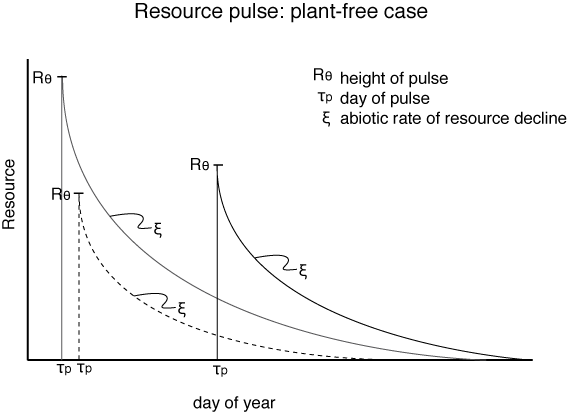
\includegraphics[width=0.8\textwidth]{/Users/Lizzie/Documents/git/temporalvar/figures/varenv_varying.png}
\caption{{\bf Major coexistence variables directly affected by
    climate change}  We focus on three major coexistence variables
  that have been (or will be) influenced by climate change---a couple
  examples of how varying them changes the resource pulse (without plants).}
\end{figure}

\newpage
\begin{figure}[h!]
\centering
\noindent 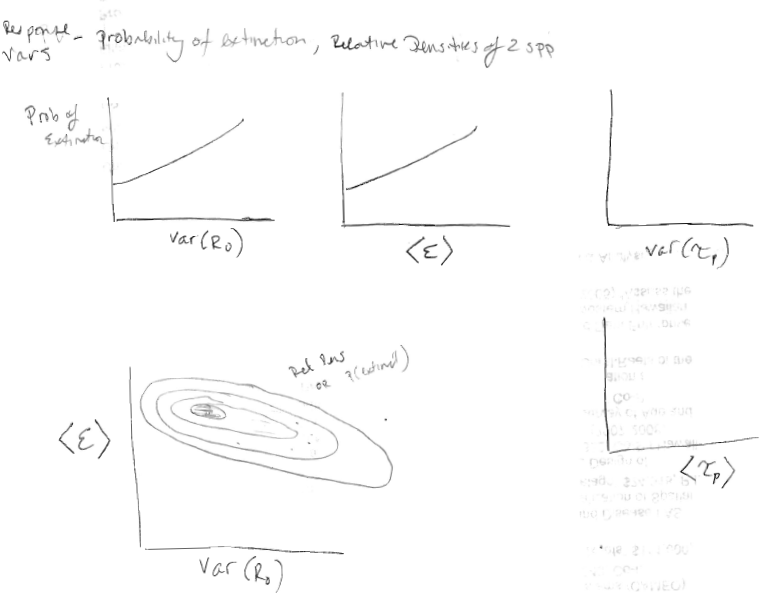
\includegraphics[width=1\textwidth]{/Users/Lizzie/Documents/git/temporalvar/figures/figurehopes_1.png}
\caption{{\bf Synergistic environmental effects.}  Figure aspirations
  for part 1 of the paper, which covers how varying environmental
  variables (\(\tau_{p}\), \(R_{\theta}\), \(\epsilon\)) alone and in concert (as predicted by climate change)
  alters coexistence. Single variables will be simple graphs, while
  contour plots will come in for varying more than one variable
  together. (There is no phenological tracking by species in this
  section of the paper.) From July 2011 meeting.}
\end{figure}

\newpage
\begin{figure}[h!]
\centering
\noindent 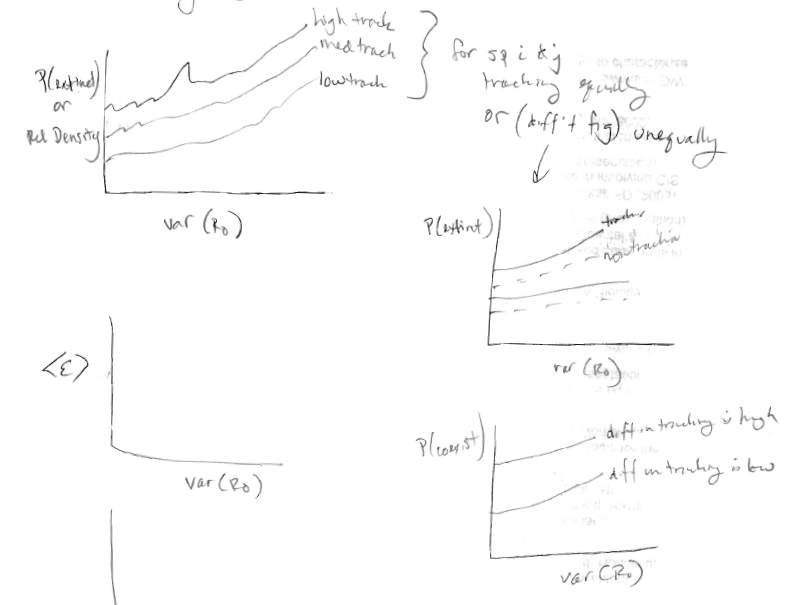
\includegraphics[width=1\textwidth]{/Users/Lizzie/Documents/git/temporalvar/figures/figurehopes_2.png}
\caption{{\bf Phenological tracking and coexistence under climate
    change.}  We didn't quite nail these down: do we vary both species
so they both track or look at one tracking and one not tracking?
Hoping this will become clear as we get the model up and running. From July 2011 meeting.}
\end{figure}



\newpage
\section{Notes from meeting with various people}

\noindent \emph{Meeting with Jenn Williams} \\

\noindent 15 October 2013\\

\noindent  There are two big areas in modeling flowering reproduction stuff in plants:
\begin{enumerate}
\item When (which year) to reproduce
\item Bet-hedging across years (how much to reproduce)
\end{enumerate}

\noindent There is not much (anything of which she is aware) of when within a year to reproduce. She pointed out that this is probably because it's easy to measure how fitness varies year to year but there not very good estimates of how fitness varies with weather a species' phenology is early or late.\\

\noindent Once she said this I though 'right!' and this jives with my reading of the literature (especially late 1970s and early 1980s, culminating a little with Ollerton \& Lack's TREE paper). But, interestingly, climate change seems to be making this issue of how fitness correlates with phenology a critical topic (and something I realized I sort of work on, ugh). Also, Jeff Diez (new prof at Riverside) is doing some of this with a snowpack study he has started in the Alps (Levine lab).\\

++\\

\noindent Most of the models include multiple decisions. And almost models to date work on death as the cost of reproduction (her and Tom Miller are actually pioneering how to model non-lethal costs such as `if I reproduce I grow less').\\

\noindent How do models handle competition? They generally include density dependence in the seedling stage. Some sort of DD is necessary for any of the ESS (evolutionary stable strategy) models and everyone just tosses it in at the seedling stage.\\

\noindent Costs vs. trade-offs: costs manifest as trade-offs in many models. She thinks we should totally just toss in a trade-off and go for it. She does this a lot, she is just sure to apply the cost at several different doses (levels) although sometimes she only presents one level.\\

++\\

\noindent She doesn't know the plasticity literature, Pigliucci (looks like he's in UT-Knoxville, I think) does some very general theory and plasticity stuff. \\

\newpage
\noindent \emph{Meeting with Sally Otto} \\

\noindent 22 October 2013\\

\noindent Okay, so she didn't really answer my costs versus trade-offs question directly. She just dove in and suggested a new formulation with costs. She felt like a model that incurred mortality when germination occurred before the pulse would be better. You could then treat \(g_{i}\) possibly as a constant or such. I pointed out that \(g_{i}\) often creates \(covar(E,C)\) but I think her model may as well, but through the intra-annual part of the equation. I think there are probably other issues with her conceptualization as well (like how we would make tracking happen) but I haven't got there yet.\\

\noindent Let:
\begin{align*}
D & = \text{normal distribution representing time of germination of species }i\\
T & = \text{intra-annual time}
\end{align*}

\noindent Then, how about this (with a less funky equation for \(g_{i}\)):

\begin{align*}
N_{i}(t+1) & =
s_{i}(N_{i}(t)(1-g_{i})+N_{i}(t)g_{i}\phi_{i}\int_{D=\tau_{p}}^{\infty}norm(\mu_{p}, \sigma_{p})_{D} [\int_{T=D}^{t+\delta}B_{i}(T) \mathrm{d}T] \mathrm{d}D)
\end{align*}

\end{document}